\documentclass[a4paper]{minimal}
\usepackage{tikz}
\usetikzlibrary{arrows}
\usetikzlibrary{decorations.pathmorphing} % wiggly line
\usetikzlibrary{positioning} % relative positioning
\usetikzlibrary{fit} % box fitting

\begin{document}
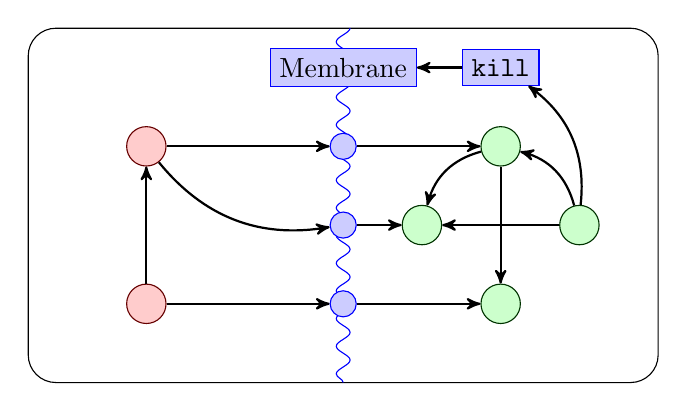
\begin{tikzpicture}[
    object/.style={circle, minimum size=5mm},
    trusted/.style={object, draw=green!20!black, fill=green!20!white},
    untrusted/.style={object, draw=red!40!black, fill=red!20},
    membrane/.style={object, draw=blue, fill=blue!20, minimum size=2mm},
    arrow/.style={thick, >=stealth'},
    pre/.style={arrow, <-},
    post/.style={arrow, ->}
  ]
  \draw[clip,rounded corners=10] (-1,0) rectangle (7,4.5);
  \node[trusted] (global) at (5,3) {};
  \node[trusted] (a) at (4,2) {}
    edge [pre,bend left] (global);
  \node[trusted] (b) at (6,2) {}
    edge [post,bend right] (global)
    edge [post] (a);
  \node[trusted] (c) at (5,1) {}
    edge [pre] (global);

  \draw[membrane,decorate,decoration=snake,fill=none] (3,0) -- (3,10);
  \node[membrane,rectangle] (membrane) at (3,4) {Membrane};
  \node[membrane,rectangle] (kill) at (5,4) {\texttt{kill}}
    edge [post] (membrane)
    edge[pre,bend left] (b);
  \node[membrane] (ma) at (3,3) {}
    edge [post] (global);
  \node[membrane] (mb) at (3,2) {}
    edge[post] (a);
  \node[membrane] (mc) at (3,1) {}
    edge [post] (c);

  \node[untrusted] (ua) at (0.5,3) {}
    edge [post] (ma)
    edge [post,bend right] (mb);
  \node[untrusted] (ub) at (0.5,1) {}
    edge [post] (ua)
    edge [post] (mc);
\end{tikzpicture}
\end{document}


